%%%%%%%%%%%%%%%%%%%%%%%%%%%%%%%%%%%%%%%%%
% Beamer Presentation
% LaTeX Template
% Version 2.0 (March 8, 2022)
%
% This template originates from:
% https://www.LaTeXTemplates.com
%
% Author:
% Vel (vel@latextemplates.com)
%
% License:
% CC BY-NC-SA 4.0 (https://creativecommons.org/licenses/by-nc-sa/4.0/)
%
%%%%%%%%%%%%%%%%%%%%%%%%%%%%%%%%%%%%%%%%%

%%%%%%%%%%%%%%%%%%%%%%%%%%%%%%%%%%%%%%%%%
% This presentation template is an adaptation of the template mentioned above. It has been created by Giovanni Spadaro and it is available on GitHub (https://github.com/Giovo17/presentation-template-unict-lm-data).
%%%%%%%%%%%%%%%%%%%%%%%%%%%%%%%%%%%%%%%%%

%----------------------------------------------------------------------------------------
%	PACKAGES AND OTHER DOCUMENT CONFIGURATIONS
%----------------------------------------------------------------------------------------

\documentclass[
	11pt, % Set the default font size, options include: 8pt, 9pt, 10pt, 11pt, 12pt, 14pt, 17pt, 20pt
	%t, % Uncomment to vertically align all slide content to the top of the slide, rather than the default centered
	%aspectratio=169, % Uncomment to set the aspect ratio to a 16:9 ratio which matches the aspect ratio of 1080p and 4K screens and projectors
]{beamer}

\graphicspath{{img/}} % Specifies where to look for included images (trailing slash required)

\usepackage{booktabs} % Allows the use of \toprule, \midrule and \bottomrule for better rules in tables

%----------------------------------------------------------------------------------------
%	SELECT LAYOUT THEME
%----------------------------------------------------------------------------------------

% Beamer comes with a number of default layout themes which change the colors and layouts of slides. Below is a list of all themes available, uncomment each in turn to see what they look like.

%\usetheme{default}
%\usetheme{AnnArbor}
%\usetheme{Antibes}
%\usetheme{Bergen}
%\usetheme{Berkeley}
%\usetheme{Berlin}
\usetheme{Boadilla}
%\usepackage{enumitem}
\usepackage{array}
%\usetheme{CambridgeUS}
%\usetheme{Copenhagen}
%\usetheme{Darmstadt}
%\usetheme{Dresden}
%\usetheme{Frankfurt}
%\usetheme{Goettingen}
%\usetheme{Hannover}
%\usetheme{Ilmenau}
%\usetheme{JuanLesPins}
%\usetheme{Luebeck}
%\usetheme{Madrid}
%\usetheme{Malmoe}
%\usetheme{Marburg}
%\usetheme{Montpellier}
%\usetheme{PaloAlto}
%\usetheme{Pittsburgh}
%\usetheme{Rochester}
%\usetheme{Singapore}
%\usetheme{Szeged}
%\usetheme{Warsaw}

%----------------------------------------------------------------------------------------
%	SELECT COLOR THEME
%----------------------------------------------------------------------------------------

% Beamer comes with a number of color themes that can be applied to any layout theme to change its colors. Uncomment each of these in turn to see how they change the colors of your selected layout theme.

%\usecolortheme{albatross}
%\usecolortheme{beaver}   % red
%\usecolortheme{beetle}
%\usecolortheme{crane}   % yellow
%\usecolortheme{dolphin}  % purple
%\usecolortheme{dove}   % white
%\usecolortheme{fly}   % grey
%\usecolortheme{lily}   % purple
%\usecolortheme{monarca}   % yellow background and black
%\usecolortheme{seagull}
%\usecolortheme{seahorse}
%\usecolortheme{spruce}   % green
\usecolortheme{whale}
%\usecolortheme{wolverine}

%----------------------------------------------------------------------------------------
%	SELECT FONT THEME & FONTS
%----------------------------------------------------------------------------------------

% Beamer comes with several font themes to easily change the fonts used in various parts of the presentation. Review the comments beside each one to decide if you would like to use it. Note that additional options can be specified for several of these font themes, consult the beamer documentation for more information.

\usefonttheme{default} % Typeset using the default sans serif font
%\usefonttheme{serif} % Typeset using the default serif font (make sure a sans font isn't being set as the default font if you use this option!)
%\usefonttheme{structurebold} % Typeset important structure text (titles, headlines, footlines, sidebar, etc) in bold
%\usefonttheme{structureitalicserif} % Typeset important structure text (titles, headlines, footlines, sidebar, etc) in italic serif
%\usefonttheme{structuresmallcapsserif} % Typeset important structure text (titles, headlines, footlines, sidebar, etc) in small caps serif

%------------------------------------------------

%\usepackage{mathptmx} % Use the Times font for serif text
\usepackage{palatino} % Use the Palatino font for serif text

%\usepackage{helvet} % Use the Helvetica font for sans serif text
\usepackage[default]{opensans} % Use the Open Sans font for sans serif text
%\usepackage[default]{FiraSans} % Use the Fira Sans font for sans serif text
%\usepackage[default]{lato} % Use the Lato font for sans serif text

%----------------------------------------------------------------------------------------
%	SELECT INNER THEME
%----------------------------------------------------------------------------------------

% Inner themes change the styling of internal slide elements, for example: bullet points, blocks, bibliography entries, title pages, theorems, etc. Uncomment each theme in turn to see what changes it makes to your presentation.

%\useinnertheme{default}
\useinnertheme{circles}
%\useinnertheme{rectangles}
%\useinnertheme{rounded}
%\useinnertheme{inmargin}

%----------------------------------------------------------------------------------------
%	SELECT OUTER THEME
%----------------------------------------------------------------------------------------

% Outer themes change the overall layout of slides, such as: header and footer lines, sidebars and slide titles. Uncomment each theme in turn to see what changes it makes to your presentation.

%\useoutertheme{default}
%\useoutertheme{infolines}
\useoutertheme{miniframes}
%\useoutertheme{smoothbars}
%\useoutertheme{sidebar}
%\useoutertheme{split}
%\useoutertheme{shadow}
%\useoutertheme{tree}
%\useoutertheme{smoothtree}

%\setbeamertemplate{footline} % Uncomment this line to remove the footer line in all slides
%\setbeamertemplate{footline}[page number] % Uncomment this line to replace the footer line in all slides with a simple slide count

%\setbeamertemplate{navigation symbols}{} % Uncomment this line to remove the navigation symbols from the bottom of all slides

% Establecer Latin Modern Sans Serif como la fuente predeterminada
\renewcommand*\familydefault{\sfdefault} % Cambia la fuente predeterminada a sans-serif
\usepackage[T1]{fontenc} % Codificación de la fuente
\usepackage{lmodern} % Carga la fuente Latin Modern\textbf{}
\usepackage{tikz}
\usetikzlibrary{positioning, arrows.meta}
\usepackage{svg}
\usetikzlibrary{calc}
\definecolor{cream}{rgb}{1,0.99,0.82} % Definición del color crema
\usetikzlibrary{positioning,fit,arrows.meta,backgrounds, shapes.geometric}

% Estilo de las cajas
\tikzset{
	boxstyle/.style={
		draw,
		thick,
		text width=2.5cm,
		minimum height=1.5cm,
		align=center
	},
	arrowstyle/.style={
		-{Latex[length=3mm]},
		thick
	}
}
%----------------------------------------------------------------------------------------
%	PRESENTATION INFORMATION
%----------------------------------------------------------------------------------------

\title[Introducción LSTM]{\textbf{Introducción a las Redes Long Short-Term Memory} \textit{(LSTM)} } % The short title in the optional parameter appears at the bottom of every slide, the full title in the main parameter is only on the title page

%\subtitle{Optional Subtitle} % Presentation subtitle, remove this command if a subtitle isn't required

\institute[]{\textit{'Jesús les habló otra vez, diciendo: «Yo soy la Luz del mundo; el que me sigue no andará en tinieblas, sino que tendrá la Luz de la vida».' \\ {\textit{Juan 8:12}}}}

\author[Rodrigo Trejo]{Rodrigo Trejo} % Presenter name(s), the optional parameter can contain a shortened version to appear on the bottom of every slide, while the main parameter will appear on the title slide


 % Your institution, the optional parameter can be used for the institution shorthand and will appear on the bottom of every slide after author names, while the required parameter is used on the title slide and can include your email address or additional information on separate lines

 % Presentation date or conference/meeting name, the optional parameter can contain a shortened version to appear on the bottom of every slide, while the required parameter value is output to the title slide

\usepackage{pgfplots}
\pgfplotsset{compat=newest}
%----------------------------------------------------------------------------------------

\begin{document}

%----------------------------------------------------------------------------------------
%	TITLE SLIDE
%----------------------------------------------------------------------------------------

\begin{frame}


	\titlepage % Output the title slide, automatically created using the text entered in the PRESENTATION INFORMATION block above
\end{frame}

%----------------------------------------------------------------------------------------
%	TABLE OF CONTENTS SLIDE
%----------------------------------------------------------------------------------------

% The table of contents outputs the sections and subsections that appear in your presentation, specified with the standard \section and \subsection commands. You may either display all sections and subsections on one slide with \tableofcontents, or display each section at a time on subsequent slides with \tableofcontents[pausesections]. The latter is useful if you want to step through each section and mention what you will discuss.

\begin{frame}
	\frametitle{Presentation Overview} % Slide title, remove this command for no title
	
	\tableofcontents % Output the table of contents (all sections on one slide)
	%\tableofcontents[pausesections] % Output the table of contents (break sections up across separate slides)
\end{frame}

%----------------------------------------------------------------------------------------
%	PRESENTATION BODY SLIDES
%----------------------------------------------------------------------------------------



\section{Limitaciones de las RNA's} % Sections are added in order to organize your presentation into discrete blocks, all sections and subsections are automatically output to the table of contents as an overview of the talk but NOT output in the presentation as separate slides

%------------------------------------------------

\begin{frame}
	\frametitle{Predicción}
	De acuerdo a las estadísticas de la Ciudad de México, si una persona mide 1.70 m, ¿Cuál será su peso en kg?
	\begin{center}
		\begin{tikzpicture}
			% Dibujo del cuadro alrededor de la red neuronal con color de fondo crema
			\fill[cream] (0,0) rectangle (4,5);
			
			% Capa de entrada
			\foreach \y in {1,2,3,4}
			\node[circle, draw, fill=blue!50] (Input-\y) at (1,\y) {};
			
			% Capa oculta
			\foreach \y [count=\s] in {1.5,2.5,3.5}
			\node[circle, draw, fill=green!50] (Hidden-\s) at (2,\y) {};
			
			% Capa de salida
			\node[circle, draw, fill=red!50] (Output) at (3,2.5) {};
			
			% Conexiones
			\foreach \y in {1,2,3,4}
			\foreach \s in {1,...,3}
			\draw[->] (Input-\y) -- (Hidden-\s);
			\foreach \s in {1,...,3}
			\draw[->] (Hidden-\s) -- (Output);
			
			% Texto de entrada y predicción con animación
			% Las flechas se extienden más allá de las paredes del rectángulo
			\draw[<-] ($(Input-2)!0.5!(Input-3)-(1.5,0)$) -- ++(-0.5,0) node[left] {\only<1->{1.70}};
			\draw[->] (Output) -- ($(Output)+(1.5,0)$) node[right] {\only<2->{80}};
		\end{tikzpicture}
	\end{center}
	
\end{frame}


\begin{frame}
	\frametitle{Clasificación}
	¿Cuál es el nombre del cantante?
	\begin{center}
		\begin{tikzpicture}
			% Dibujo del cuadro alrededor de la red neuronal con color de fondo crema
			\fill[cream] (0,0) rectangle (4,5);
			
			% Capa de entrada
			\foreach \y in {1,2,3,4}
			\node[circle, draw, fill=blue!50] (Input-\y) at (1,\y) {};
			
			% Capa oculta
			\foreach \y [count=\s] in {1.5,2.5,3.5}
			\node[circle, draw, fill=green!50] (Hidden-\s) at (2,\y) {};
			
			% Capa de salida
			\node[circle, draw, fill=red!50] (Output) at (3,2.5) {};
			
			% Conexiones
			\foreach \y in {1,2,3,4}
			\foreach \s in {1,...,3}
			\draw[->] (Input-\y) -- (Hidden-\s);
			\foreach \s in {1,...,3}
			\draw[->] (Hidden-\s) -- (Output);
			
			% Imagen de entrada más grande y más a la izquierda con animación
			\uncover<1->{
				\node[left=3.5cm of Input-2.center, anchor=center] (image) {
\includegraphics[width=.25\textwidth]{maluma.png}};
			}
			
			% Flecha apuntando a las neuronas de entrada
			\draw[->] ([xshift=-2cm]$(Input-2)!.5!(Input-3)$) -- ($(Input-2)!.5!(Input-3)$);
			
			% Texto de predicción con animación
			\uncover<2->{
				\draw[->] (Output) -- ($(Output)+(1.5,0)$) node[right] {Maluma};
			}
		\end{tikzpicture}
	\end{center}
\end{frame}

%------------------------------------------------

\begin{frame}
	\frametitle{¿Secuencias?}
	\vspace{-2mm}
	Angelito va en el metro camino a su casa y se encuentra en esta estación... \textit{¿Cuál es la siguiente?}
	\vspace{8mm}
	
	\begin{tikzpicture}[node distance=2cm and 0cm]
		% Dibujo del cuadro alrededor de la red neuronal con color de fondo crema y esquinas redondeadas
		% Ajustar el rectángulo para que sea más estrecho y no tan ancho
		\fill[cream, rounded corners] (3,0.5) rectangle (8,4.5); % Se ajusta para ser más estrecho
		
		% Capa de entrada, centrada dentro del cuadro crema
		\foreach \y in {1,2,3,4}
		\node[circle, draw, fill=blue!50] (Input-\y) at (4,\y) {};
		
		% Capa oculta, centrada dentro del cuadro crema
		\foreach \y [count=\s] in {1.5,2.5,3.5}
		\node[circle, draw, fill=green!50] (Hidden-\s) at (5.5,\y) {};
		
		% Capa de salida, centrada dentro del cuadro crema
		\node[circle, draw, fill=red!50] (Output) at (7,2.5) {};
		
		% Conexiones
		\foreach \y in {1,2,3,4}
		\foreach \s in {1,...,3}
		\draw[->] (Input-\y) -- (Hidden-\s);
		\foreach \s in {1,...,3}
		\draw[->] (Hidden-\s) -- (Output);
		
		% Imagen de entrada, centrada con respecto a la red neuronal
		\uncover<2->{
			\node[anchor=center] (image) at (1cm,2.5cm) {
\includegraphics[width=.2\textwidth]{pinosuarez.png}};
		}
		
		% Flecha desde la imagen de entrada a las neuronas de entrada
		\uncover<2->{
			\draw[->] (image.east) -- ($(Input-2)!.5!(Input-3)$);
		}
		
		% Imagen de predicción, movida más hacia la derecha
		\uncover<3->{
			\node[right=3cm of Output.center, anchor=center] (prediccion) {
\includegraphics[width=.25\textwidth]{esponja.jpeg}};
		}
		
		% Flecha desde la capa de salida a la imagen de predicción
		\uncover<3->{
			\draw[->] (Output) -- (prediccion.west);
		}
	\end{tikzpicture}

\end{frame}


\begin{frame}
	\frametitle{¿Secuencias?}
	¿Qué debería conocer la Red Neuronal para poder decir qué estación sigue?
	
	\begin{columns}
		\begin{column}{0.5\textwidth}
			\begin{center}
				
\includegraphics[width=0.5\linewidth]{bat.jpg}
			\end{center}
		\end{column}
		\begin{column}{0.5\textwidth}
			\begin{itemize}
				\item<2-> Saber en qué linea está.
				\item<3-> \textit{\textbf{Recordar}} en qué línea está.
				\item<4-> \textbf{\textit{Recordar}} en qué estaciones estuvo antes (para deducir la linea).
				\item<5-> TENER MEMORIA.
			\end{itemize}
		\end{column}
	\end{columns}
\end{frame}





%------------------------------------------------



\section{Plan de Trabajo}

\begin{frame}
	\frametitle{Cronograma}
	
	\begin{table}[h]
		\centering
		\begin{tabular}{|l|p{8cm}|}
			\hline
			Semana & Temática \\ \hline
			25-29/03 & Resumen, Plan de trabajo y preparación del set de datos \\ \hline
			01-05/04 & Introducción a las Redes Neuronales Artificiales, Redes LSTM, y creación de los modelos de las variables ambientales\\ \hline
			08-12/04 & Construcción, entrenamiento y prueba del modelo de predicción de ingresos hospitalarios \\ \hline
		\end{tabular}
		\caption{Planificación del curso por semana}
		\label{table:plan_semanal1}
	\end{table}

\end{frame}

%------------------------------------------------

\begin{frame}
	\frametitle{Cronograma}
	
	\begin{table}[h]
		\centering
		\begin{tabular}{|l|p{8cm}|}
			\hline
			Semana & Temática \\ \hline
			15-19/04 & Modificaciones y variantes del modelo principal. Elección del mejor modelo\\ \hline
			22-26/04 & Resolución y ajustes finales  \\ \hline
		\end{tabular}
		\caption{Planificación del curso por semana}
		\label{plan_semanal2}
	\end{table}


\end{frame}

%------------------------------------------------



\section{Entrenamiento de una RNA}


\begin{frame}
	\frametitle{Backpropagation: Corrección de erroes}
	\begin{center}
		\begin{tikzpicture}[scale=0.7, transform shape, >=Stealth]
			% Estilos de nodos
			\tikzset{
				neuron/.style={circle,fill=black!25,minimum size=22pt,inner sep=0pt},
				input neuron/.style={neuron, fill=green!50},
				output neuron/.style={neuron, fill=red!50, align=center},
				hidden neuron/.style={neuron, fill=blue!50, align=center},
				annot/.style={text width=4em, text centered}
			}
			
			% Dibuja la capa de entrada
			\foreach \name / \y in {1,...,2}
			\node[input neuron] (I-\name) at (0,-\y*2.5) {$x_{\name}$};
			
			% Dibuja la capa oculta
			\foreach \name / \y in {1,...,3}
			\node[hidden neuron] (H-\name) at (5cm,-\y*2.5) {$\sigma$};
			
			% Dibuja la capa de salida
			\node[output neuron,pin={[pin edge={->}]right:$\hat{y}$}, right=of H-2] (O) {$\sigma$};
			
			% Conecta las unidades con pesos
			\foreach \source in {1,...,2} {
				\foreach \dest in {1,...,3} {
					\draw (I-\source) -- (H-\dest) node[midway, above, sloped, pos=0.7, xshift=(\source-1.5)*3pt, yshift=(\dest-2)*3pt] {$w_{\source,\dest}$};
				}
			}
			
			% Conecta la capa oculta a la de salida con pesos
			\foreach \source in {1,...,3} {
				\pgfmathtruncatemacro{\result}{\source}
				\draw (H-\source) -- (O) node[midway, above, sloped, yshift=\source*2pt] {$w_{\result,1}$};
			}
			
			% Etiquetas
			\node[annot,above=of H-1, yshift=0.1cm] {Capa oculta};
			\node[annot,left=of I-1, node distance=3cm] (capa_entrada) {Capa de entrada};
			\node[annot,right=of O, node distance=3cm] {Capa de salida};
			
			% Dibuja el vector columna debajo de la etiqueta "Capa de entrada"
			\node[below=0.5cm of capa_entrada] (vector) {${\vec{\mathbf{X}}} = \begin{bmatrix} x_1 \\ x_2 \\ \vdots \\ x_n \end{bmatrix}$};
			
			% Conexiones de vector columna
			\draw[->] (vector) -- (I-1);
			\draw[->] (vector) -- (I-2);
			
			% Sesgo
			\node[above=0.5cm of H-2] (Bias) {$b$};
			\draw[->] (Bias) -- (H-2);
			
			% Flecha "forward"
			% Flecha "Forward" controlada manualmente
			\draw[->, thick] (8, -9) -- node[above] {Backpropagation} (-1, -9);
		\end{tikzpicture}
	\end{center}
	
	
\end{frame}


\begin{frame}
	\frametitle{Función de Error (MSE)}
	
	\textbf{MSE: Mean Square Error}
	
	\begin{block}{Expresión Matemática}
		La fórmula para calcular el MSE es:
		\[ MSE = \frac{1}{n} \sum_{i=1}^{n} (Y_{i} - \hat{Y}_{i})^2 \]
		donde:
		\begin{itemize}
			\item $n$ es el número total de observaciones (o ejemplos de entrenamiento),
			\item $Y_{i}$ es el valor real del i-ésimo ejemplo,
			\item $\hat{Y}_{i}$ es la predicción del modelo para el i-ésimo ejemplo.
		\end{itemize}
	\end{block}
	
\end{frame}

\begin{frame}
	\frametitle{Función de Error (MSE)}
	\begin{block}{Explicación: ¿Qué hace el MSE?}
		El MSE mide el promedio de los cuadrados de los errores; es decir, la diferencia cuadrática promedio entre los valores estimados y los valores reales. Al elevar al cuadrado las diferencias:
		\begin{itemize}
			\item Penaliza más fuertemente los errores grandes, lo que puede ser deseable en muchos casos.
			\item Asegura que solo tengamos valores positivos, simplificando el análisis de los errores.
		\end{itemize}
		Esto lo convierte en una herramienta poderosa para guiar al modelo en el proceso de aprendizaje, buscando minimizar estas diferencias y, por ende, el error de predicción.
	\end{block}
\end{frame}

\begin{frame}
	\frametitle{Función de Error (MSE)}
	\begin{block}{¿Por qué es importante el MSE?}
		Una función de error baja indica que el modelo tiene una buena precisión en sus predicciones. Reducir el MSE es fundamental en el proceso de optimización del modelo, llevándolo a hacer predicciones cada vez más cercanas a los valores reales.
	\end{block}
\end{frame}

\begin{frame}
	\frametitle{Resumen}
	
	\begin{table}[h]
		\centering
		\begin{tabular}{|l|p{6cm}|c|}
			\hline
			Elemento & Descripción & Origen \\ \hline
			Entradas ($\vec{x}$) & Variables de entrada proporcionadas al modelo (por ejemplo, características de los datos de entrada) & P \\ \hline
			Pesos ($\vec{\mathbf{W}}$) & Parámetros aprendidos por el modelo durante el entrenamiento & C \\ \hline
			Sesgo ($\vec{b}$) & Término aditivo introducido para ajustar la salida de cada neurona & P \\ \hline
			Función de activación & Función aplicada a la salida de cada neurona para introducir no linealidades en el modelo & P \\ \hline
		\end{tabular}
		\caption{Elementos básicos de una red neuronal (Parte 1)}
		\label{table:elementos_red_neuronal1}
	\end{table}
	
\end{frame}

\begin{frame}
	\frametitle{Resumen}
	
	\begin{table}[h]
		\centering
		\begin{tabular}{|l|p{6.5cm}|c|}
			\hline
			Elemento & Descripción & Origen \\ \hline
			Función de error & Función que mide la discrepancia entre las predicciones del modelo y los valores reales & P \\ \hline
			Capas ocultas & Capas intermedias entre la capa de entrada y la capa de salida que contienen neuronas & P \\ \hline
			Neuronas por capa & Número de unidades de procesamiento en cada capa oculta & P \\ \hline
			Predicción ($\hat{y}$) & Valor calculado por el modelo como salida final & C \\ \hline
			Target ($y$) & Valor real al que se compara la predicción durante el entrenamiento & P \\ \hline
		\end{tabular}
		\caption{Elementos básicos de una red neuronal (Parte 2)}
		\label{table:elementos_red_neuronal2}
	\end{table}
\end{frame}

\begin{frame}
	\frametitle{Resumen}
	\begin{center}
		{\large Entrenar una Red Neuronal implica aplicar el método de \textit{Prueba y Error}. Es un algoritmo que nos puede ayudar a dominar el arte de tener paciencia.}
		
		\vspace{5mm}
		
		
\includegraphics[width=3.8cm]{cerveza.jpg}
		
	\end{center}
	
\end{frame}


\begin{frame}
	\frametitle{Entrenamiento de una RNA}
	
	\textit{\textbf{Objetivo:} Minimizar la función de error.}
	\vspace{3mm}
	
	¿CÓMO?
	\vspace{3mm}
	
	\begin{itemize}
		\item Aplicando derivadas
		\item Para el caso de una función multivariable: \textbf{Aplicando el gradiente}
		\item Como es difícil usar un método analítico (con fórmulas) para determinar el mínimo de la función de error:
		\begin{itemize}
			\item Aplicamos un método numérico iterativo conocido como: \textit{\textbf{Descenso de gradiente.}}
		\end{itemize}
	\end{itemize}
        
 
\end{frame}

%------------------------------------------------

\begin{frame}
	\frametitle{Descenso de gradiente - El parámetro learning\_rate ($\alpha$)}
	
     \begin{center}
     	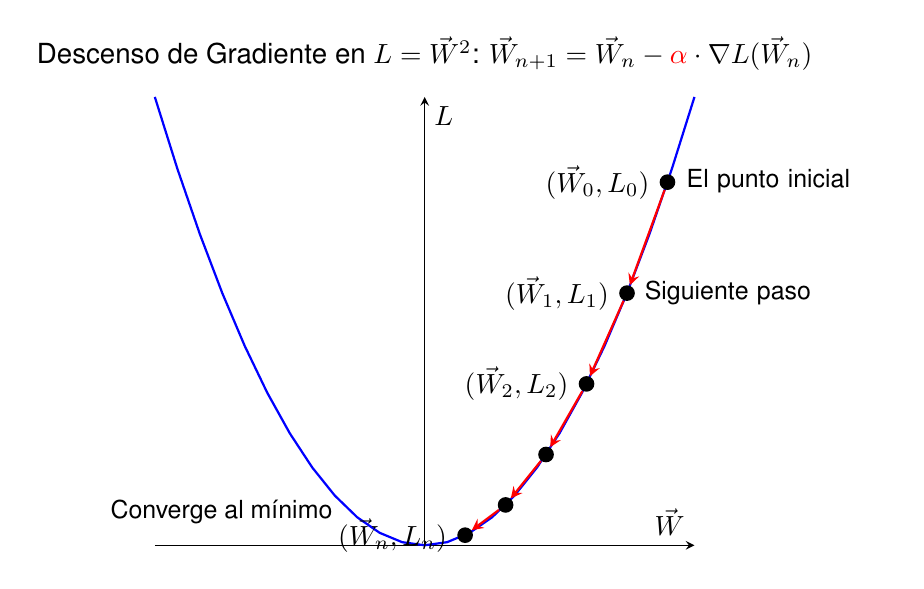
\begin{tikzpicture}
     		\begin{axis}[
     			title={Descenso de Gradiente en $L = \vec{W}^2$: $\vec{W}_{n+1} = \vec{W}_n - \textcolor{red}{\alpha} \cdot \nabla L(\vec{W}_n)$},
     			xlabel={$\vec{W}$},
     			ylabel={$L$},
     			axis lines=middle,
     			xmin=-2, xmax=2,
     			ymin=0, ymax=4,
     			ticks=none,
     			clip=false,
     			]
     			
     			% Dibuja la función
     			\addplot[blue, thick, domain=-2:2] {x^2};
     			
     			% Puntos y flechas del descenso de gradiente
     			\node<2->[label={180:{$(\vec{W}_0,L_0)$}},circle,fill,inner sep=2pt] (start) at (axis cs:1.8,{1.8^2}) {};
     			\node<3->[label={180:{$(\vec{W}_1,L_1)$}},circle,fill,inner sep=2pt] (mid1) at (axis cs:1.5,{1.5^2}) {};
     			\node<4->[label={180:{$(\vec{W}_2,L_2)$}},circle,fill,inner sep=2pt] (mid2) at (axis cs:1.2,{1.2^2}) {};
     			\node<5->[circle,fill,inner sep=2pt] (mid3) at (axis cs:0.9,{0.9^2}) {};
     			\node<6->[circle,fill,inner sep=2pt] (mid4) at (axis cs:0.6,{0.6^2}) {};
     			\node<7->[label={180:{$(\vec{W}_n,L_n)$}},circle,fill,inner sep=2pt] (end) at (axis cs:0.3,{0.3^2}) {};
     			
     			% Flechas entre los puntos
     			\draw<3->[-stealth, red, thick] (start) -- (mid1);
     			\draw<4->[-stealth, red, thick] (mid1) -- (mid2);
     			\draw<5->[-stealth, red, thick] (mid2) -- (mid3);
     			\draw<6->[-stealth, red, thick] (mid3) -- (mid4);
     			\draw<7->[-stealth, red, thick] (mid4) -- (end);
     			
     			% Anotaciones
     			\node<2->[align=center, font=\small, text width=3cm, anchor=west] at (axis cs:1.6,3.25) 
     			{El punto inicial};
     			\node<3->[align=center, font=\small, text width=3cm, anchor=west] at (axis cs:1.3,2.25) 
     			{Siguiente paso};
     			\node<7->[align=center, font=\small, anchor=west] at (axis cs:-2.4,0.3) 
     			{Converge al mínimo};
     			
     		\end{axis}
     	\end{tikzpicture}
     \end{center}
 
\end{frame}

%------------------------------------------------

\begin{frame}
	\frametitle{Cuando $\alpha$ es muy pequeño}
	
	\begin{center}
		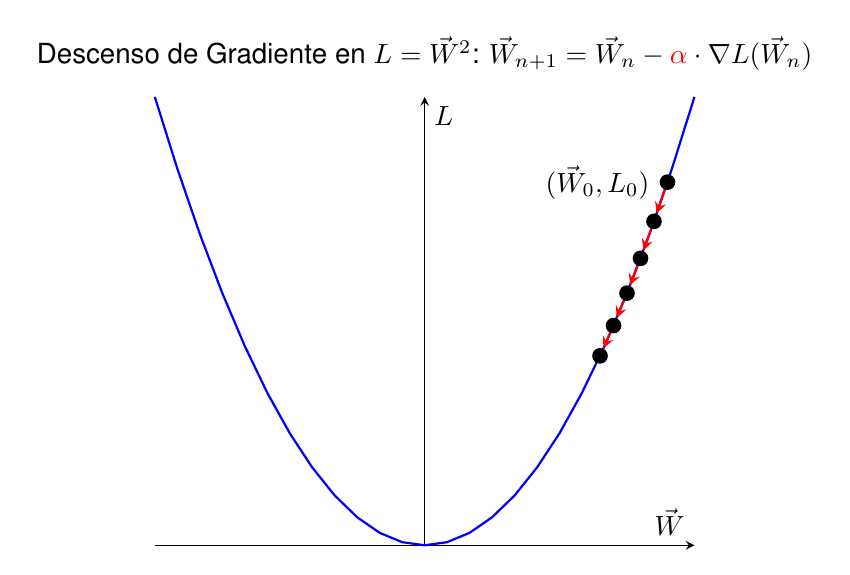
\begin{tikzpicture}
			\begin{axis}[
				title={Descenso de Gradiente en $L = \vec{W}^2$: $\vec{W}_{n+1} = \vec{W}_n - \textcolor{red}{\alpha} \cdot \nabla L(\vec{W}_n)$},
				xlabel={$\vec{W}$},
				ylabel={$L$},
				axis lines=middle,
				xmin=-2, xmax=2,
				ymin=0, ymax=4,
				ticks=none,
				clip=false,
				]
				
				% Dibuja la función
				\addplot[blue, thick, domain=-2:2] {x^2};
				
				% Puntos y flechas del descenso de gradiente
				\node[label={180:{$(\vec{W}_0,L_0)$}},circle,fill,inner sep=2pt] (start) at (axis cs:1.8,{1.8^2}) {};
				
				\node[label={180:{}},circle,fill,inner sep=2pt] (mid1) at (axis cs:1.7,{1.7^2}) {};
				
				\node[label={180:{}},circle,fill,inner sep=2pt] (mid2) at (axis cs:1.6,{1.6^2}) {};
				
				\node[label={180:{}},circle,fill,inner sep=2pt] (mid3) at (axis cs:1.5,{1.5^2}) {};
				
				\node[label={180:{}},circle,fill,inner sep=2pt] (mid4) at (axis cs:1.4,{1.4^2}) {};
				
				\node[label={180:{}},circle,fill,inner sep=2pt] (end) at (axis cs:1.3,{1.3^2}) {};
					
				% Flechas entre los puntos
				\draw[-stealth, red, thick] (start) -- (mid1);
				\draw[-stealth, red, thick] (mid1) -- (mid2);
				\draw[-stealth, red, thick] (mid2) -- (mid3);
				\draw[-stealth, red, thick] (mid3) -- (mid4);
				\draw[-stealth, red, thick] (mid4) -- (end);
				
			\end{axis}
		\end{tikzpicture}
	\end{center}"
	
\end{frame}


\begin{frame}
	\frametitle{Cuando $\alpha$ es muy grande}
	
	\begin{center}
		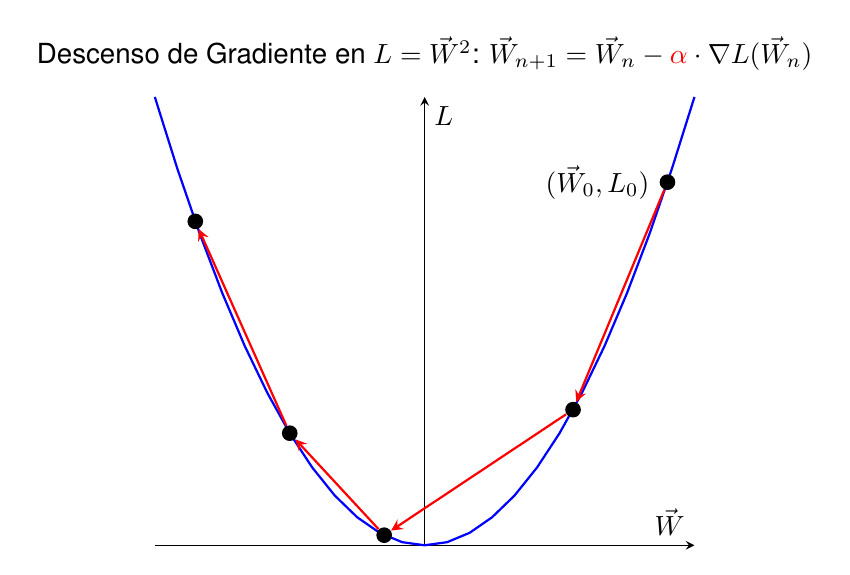
\begin{tikzpicture}
			\begin{axis}[
				title={Descenso de Gradiente en $L = \vec{W}^2$: $\vec{W}_{n+1} = \vec{W}_n - \textcolor{red}{\alpha} \cdot \nabla L(\vec{W}_n)$},
				xlabel={$\vec{W}$},
				ylabel={$L$},
				axis lines=middle,
				xmin=-2, xmax=2,
				ymin=0, ymax=4,
				ticks=none,
				clip=false,
				]
				
				% Dibuja la función
				\addplot[blue, thick, domain=-2:2] {x^2};
				
				% Puntos y flechas del descenso de gradiente
				\node[label={180:{$(\vec{W}_0,L_0)$}},circle,fill,inner sep=2pt] (start) at (axis cs:1.8,{1.8^2}) {};
				
				\node[label={180:{}},circle,fill,inner sep=2pt] (mid1) at (axis cs:1.1,{1.1^2}) {};
				
				\node[label={180:{}},circle,fill,inner sep=2pt] (mid2) at (axis cs:-0.3,{(-0.3)^2}) {};
				
				\node[label={180:{}},circle,fill,inner sep=2pt] (mid3) at (axis cs:-1,{(-1)^2}) {};
				
				\node[label={180:{}},circle,fill,inner sep=2pt] (end) at (axis cs:-1.7,{(-1.7)^2}) {};
				
				
				% Flechas entre los puntos
				\draw[-stealth, red, thick] (start) -- (mid1);
				\draw[-stealth, red, thick] (mid1) -- (mid2);
				\draw[-stealth, red, thick] (mid2) -- (mid3);
				\draw[-stealth, red, thick] (mid3) -- (end);
				
			\end{axis}
		\end{tikzpicture}
	\end{center}
	
\end{frame}

\begin{frame}
	\begin{center}
		Y si... el learning\_rate también lo define el programador /:
		\vspace{5mm}
		
		
\includegraphics[width=6cm]{gato.jpeg}
	\end{center}
\end{frame}

\begin{frame}
	\frametitle{Ejemplito: Compuerta XOR}
	\vspace{-5mm}
	\begin{columns}
		\begin{column}{0.5\textwidth}
			\begin{center}
				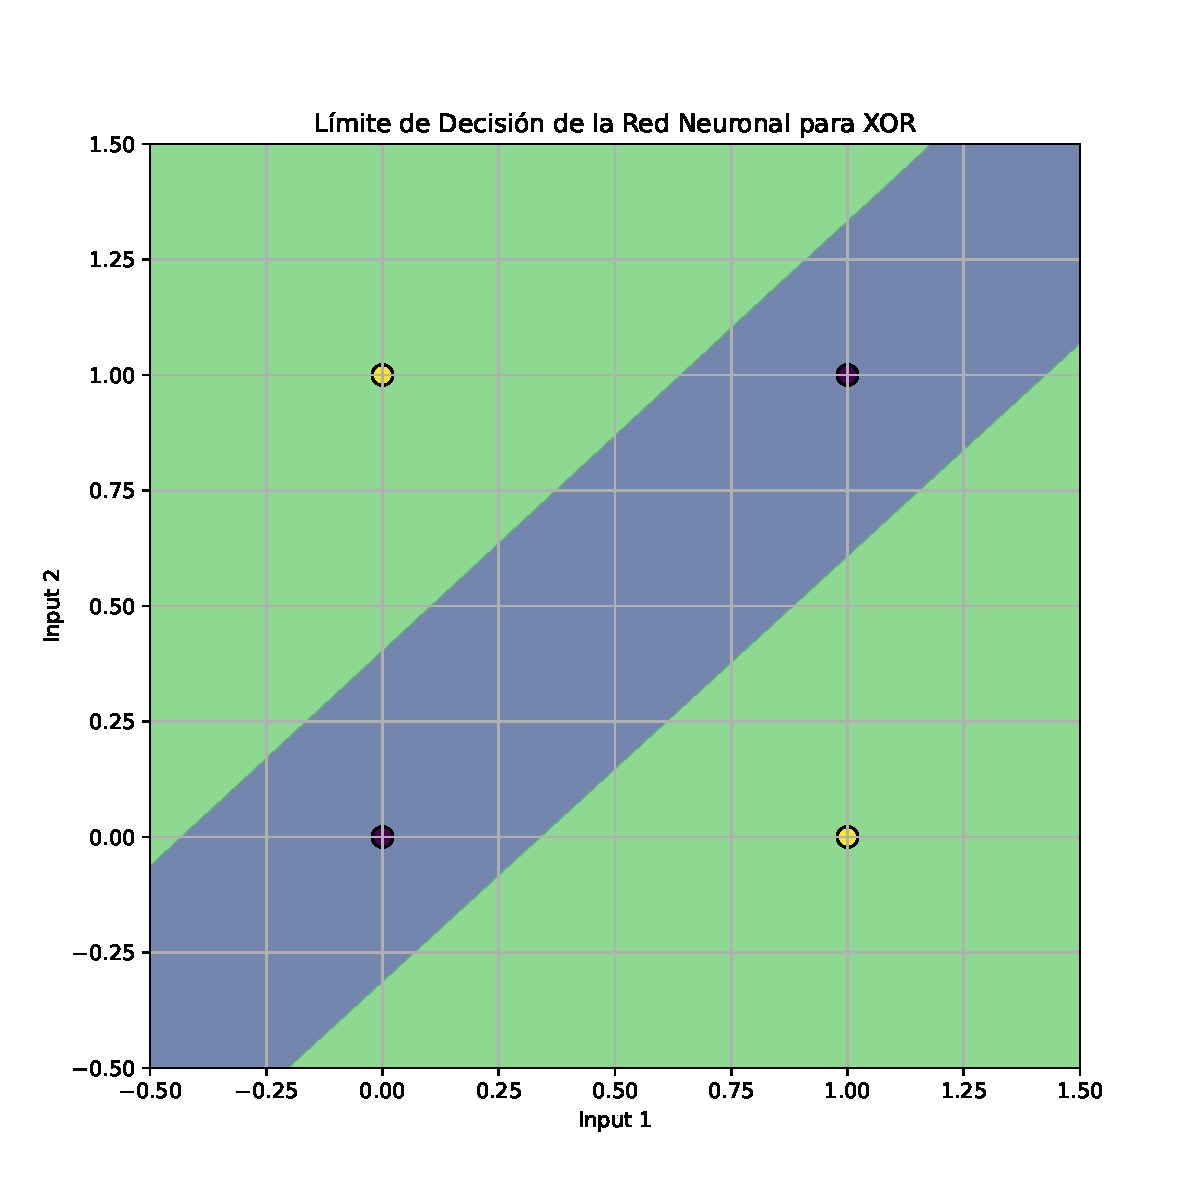
\includegraphics[width=0.6\linewidth]{xor1.pdf}
			\end{center}
		\end{column}
		\begin{column}{0.5\textwidth}
			\begin{center}
				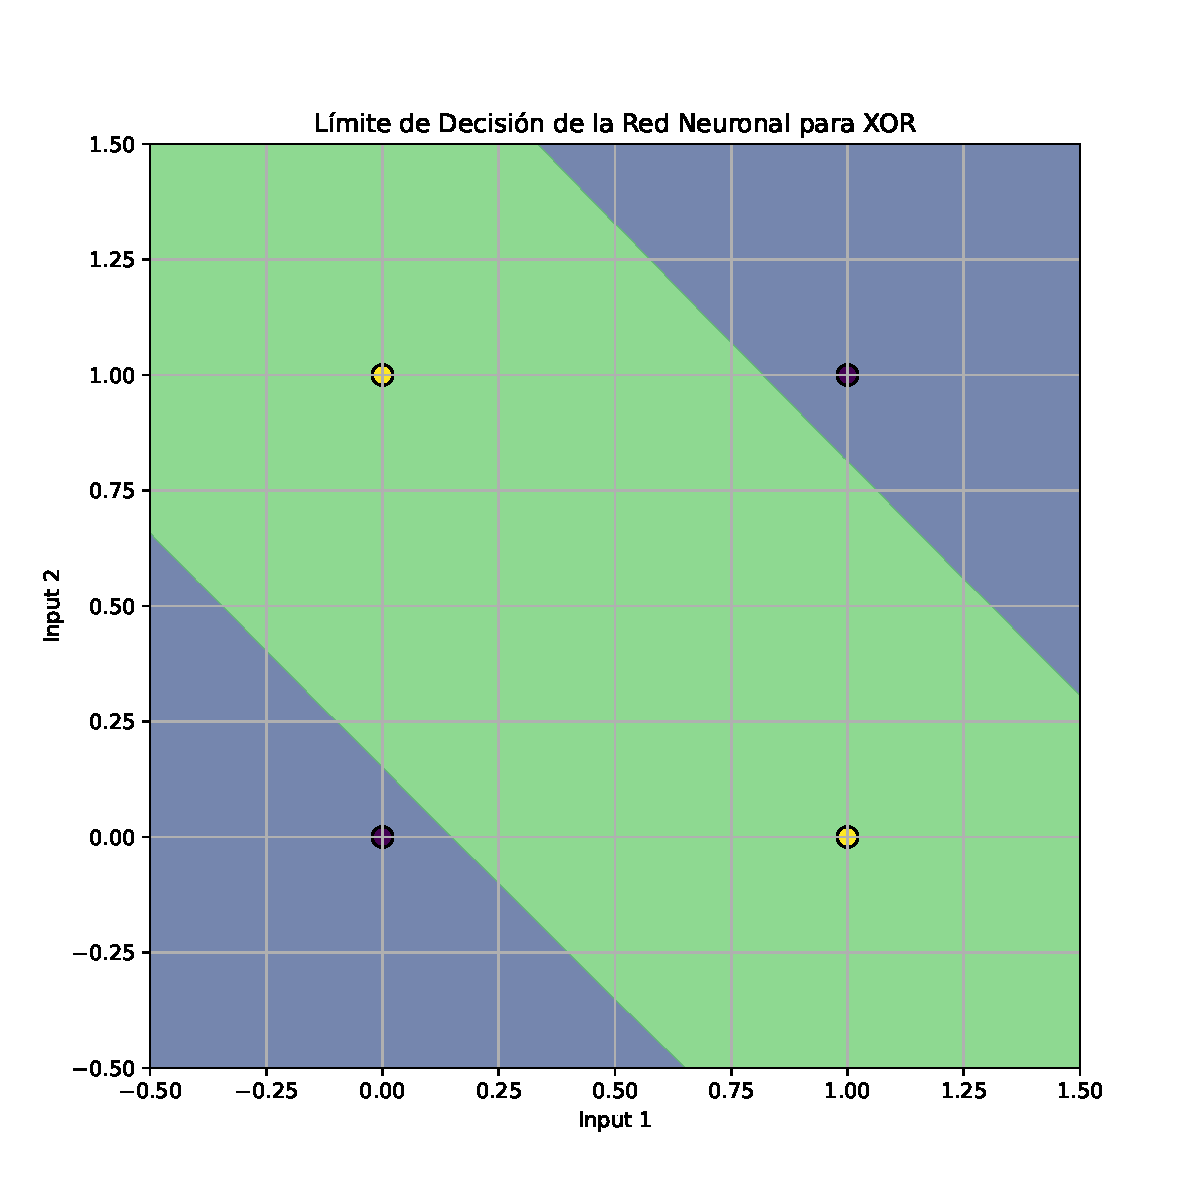
\includegraphics[width=0.6\linewidth]{xor2.pdf}
			\end{center}
		\end{column}
	\end{columns}

	
	\begin{columns}
		\begin{column}{0.5\textwidth}
			\begin{center}
				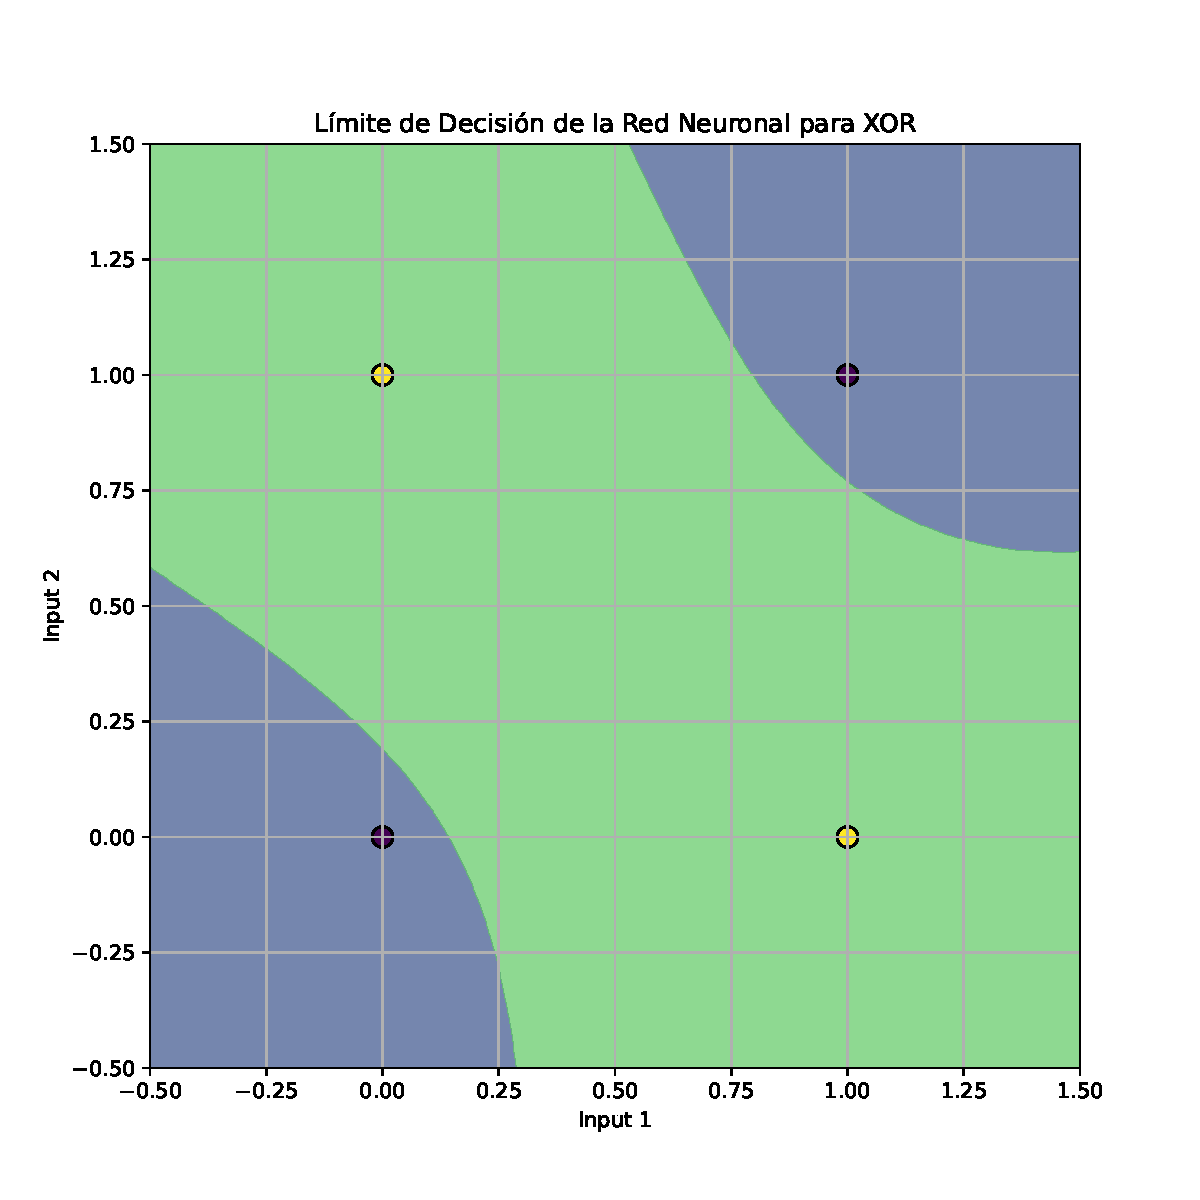
\includegraphics[width=0.6\linewidth]{xor3.pdf}
			\end{center}
		\end{column}
		\begin{column}{0.5\textwidth}
			\begin{center}
				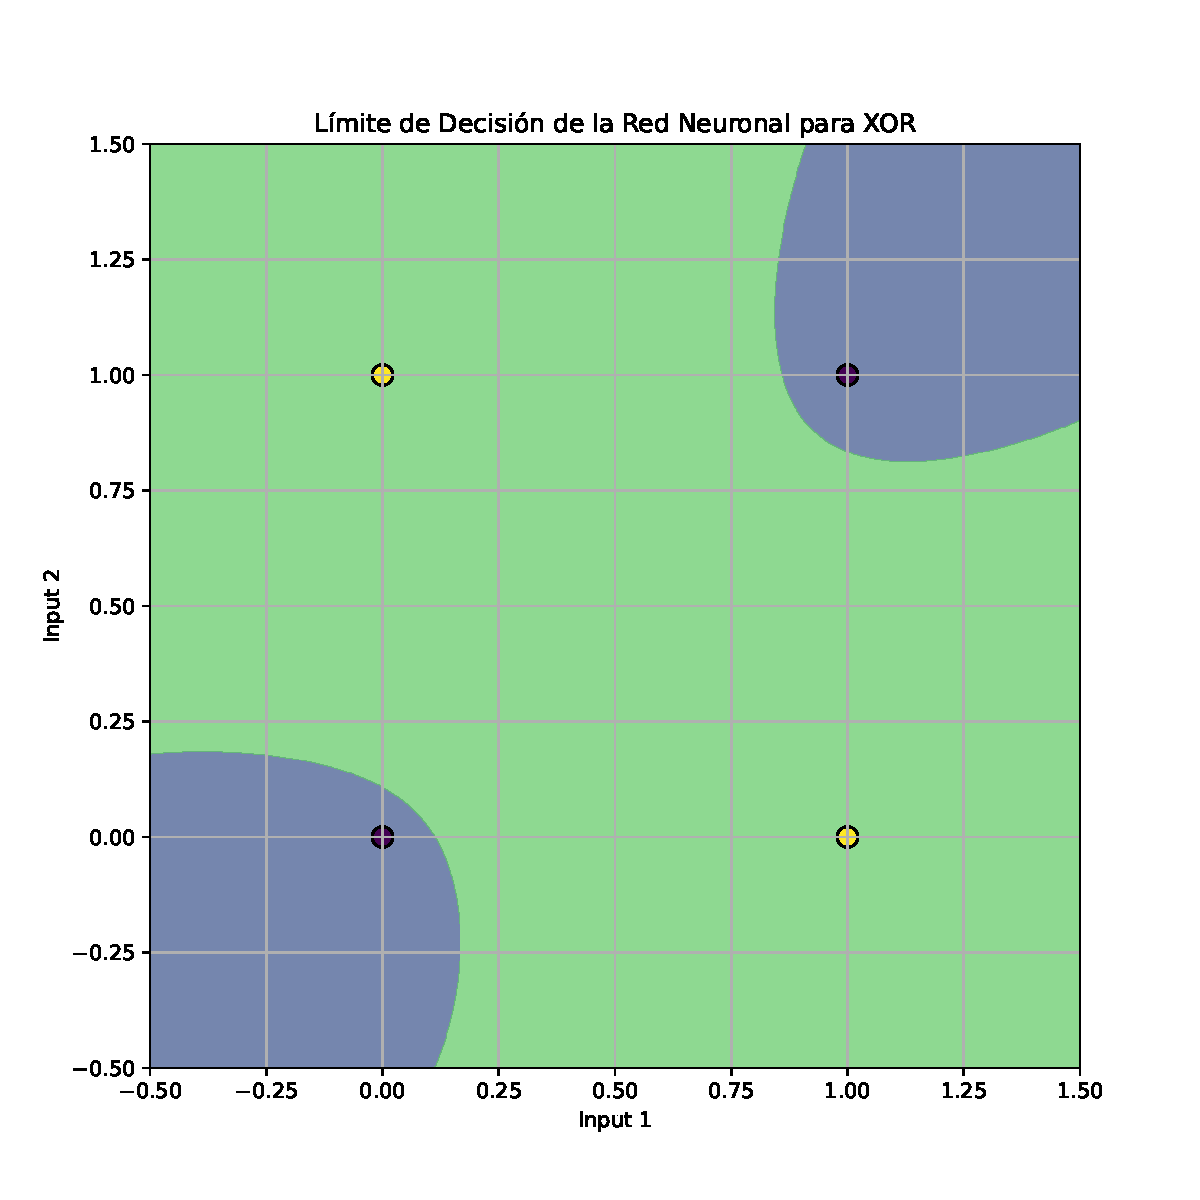
\includegraphics[width=0.6\linewidth]{xor4.pdf}
			\end{center}
		\end{column}
	\end{columns}
\end{frame}



%----------------------------------------------------------------------------------------
%	CLOSING SLIDE
%----------------------------------------------------------------------------------------

\begin{frame}[plain] % The optional argument 'plain' hides the headline and footline
	\begin{center}
		\vspace{15mm}
		{\Huge ¡Gracias!}
		
		
        
\includegraphics[width=5cm]{tortuga.png}
	\end{center}
\end{frame}

%----------------------------------------------------------------------------------------

\end{document} 